\ylDisplay{Keha vees} % Ülesande nimi
{Jonatan Kalmus} % Autor
{lõppvoor} % Voor
{2019} % Aasta
{P 8} % Ülesande nr.
{3} % Raskustase
{
% Teema: Mehaanika

\ifStatement
Joonisel on lennuki algne asukoht märgitud ristiga. Iga tunni järel mõõdeti lennuki kaugust fikseeritud punktist. Saadud kaugused on joonisel märgitud ringjoonena mõõtepunkti ümber. Konstrueerida kõik võimalikud lennuki trajektoorid $7$ h jooksul, kui on teada, et pärast starti lendas lennuk $4$ h otse, muutis seejärel suunda ning lendas ülejäänud aja samuti otse. Eeldada, et lennuki kiirus maapinna suhtes oli ühtlaselt $500$ km/h. Lahendus esitage lisalehel. NB! Suuna muutus võis olla ka väga väike.
\begin{center}
	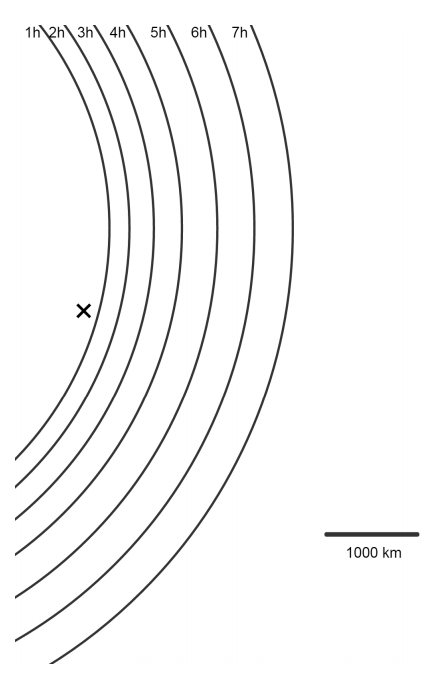
\includegraphics[width=0.5\linewidth]{2019-v3p-08-yl.PNG}
\end{center}
\fi

\ifHint
Joonisel oleva mõõtkava järgi saab võtta $500$ km vastava pikkuse joonisel. See pikkus tuleb võtta sirkli haarade vahele ja joonestada vastava raadiusega ringjooni märkides sirgjoonega lennuki võimalikke trajektoore.
\fi

\ifSolution
Teame, et suured ringjooned märgivad lennuki asukohta iga tunni järel ning ühe tunniga läbib lennuk $500$ km. Joonisel oleva mõõtkava järgi saame $500$ km vastava pikkuse joonisel. Võtame selle pikkuse ja joonestame sirkliga vastava raadiusega ringjoone lennuki algasukoha ümber. See ringjoon märgib lennuki asukohta $1$ h pärast õhkutõusu ning selle lõikepunktid olemasoleva esimese suure ringjoonega (mis märgib samuti lennuki asukohta $1$ h pärast õhkutõusu) annavad meile lennuki võimalikud asukohad $1$ h pärast. Kuna me ei tea, millises suunas lennuk lendas, peame lennuki teekonda mõlemast punktist edasi konstrueerima, joonestades uute punktide ümber samuti 500km vastava ringjoone. Kuna aga teame, et lennuk lendas $4$ h järjest otse, saame hakata lõikepunkte välistama, sest sobivad punktid moodustavad sirge. $4$ h vastava ringjoone juures teame vaid seda, et lennuk muutis suunda. Seega saame kummagi algse teekonna kohta veel 2 võimalikku uut suunda (kokku 4 võimalikku suunda). Teades, et lennuk lendas edaspidi samuti vaid otse, saame kõik 4 teekonda lõpuni konstrueerida.
\begin{center}
	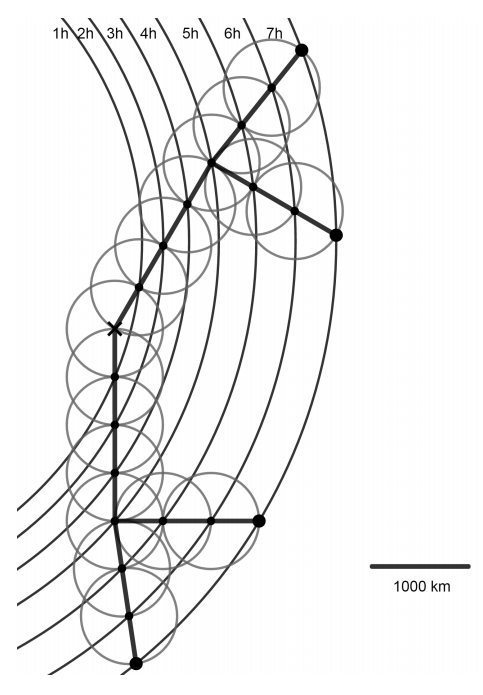
\includegraphics[width=0.5\linewidth]{2019-v3p-08-lah.PNG}
\end{center}
\fi
}
 
